\chapter{Analysis}

In this chapter, we will be doing problem analysis. We will dive deeper into the problem we intend to fix, and why we believe it to be a problem in the first place. We also compare source code with our definition of pseudocode, to get a better feel for their differences. Lastly, we will discuss some of the existing approaches briefly mentioned in Section 2.1.1 and 2.1.2, which solve parts of the problem.

\section{Problem Definition}

Now is as good a time as any to outline the problem at hand more concretely. Simply put, we aim to present computer programs at different abstraction levels, whilst maintaining their underlying ideas. The concept is nothing new, but has traditionally been carried out manually by the programmer. We believe there is a benefit in centralising resources and automating the conversion part. \\

There are several use cases where it is useful to display source code in a different light. Mainly within education, where the goal is to teach students concepts in an agonstic way. However, it could also be used by researchers exchanging ideas, across preferred programming languages. \\

Already in the 1980's Clements et al. predicted that computers would be an integral part of the classroom~\cite{computersInTheClassroom}. Slowly but surely also the art of computer programming has been introduced into school curriculums, at an increasingly younger age. \\

\forsup{Bør jeg kildeføre det siste anvsittet der?}

Admittedly, instructing 10-year-olds in complex concepts like pointers and multi-threading may not be the most effective use of time. However, there is value in familiarizing them with computer programming, which is a fundamental aspect of our increasingly digital world. \\

\forsup{Det siste er vel en påstand, er det ok?}

If a teacher transpiles their code to flowcharts, it offers a visual approach to understanding programming concepts. Subsequently, the whole classroom can focus on the underlying logic than on the syntactic quirks of the teacher's preferred programming language. \\

This is also the case when teaching computer programs at a higher level, like in university. Opting for pseudocode instead of a specific programming language levels the playing field, as well as helping students coming from a mathematical background. \\

\forsup{Tanken er at, som feks i IN2010, så får man (til en viss grad) velge språk selv. Så om man ikke er god i Java, så slipper man at alle eksemplene er med Java. I tillegg kan de fra matte, med en svakere programmeringsbakgrunn få litt drahjelp, da pseudokode gjerne benytter litt matematisk notasjon}

Lastly, researchers might wish to exchange ideas despite using different programming languages. Just like every animal in the kingdom can be called upon in latin, all computer programs can be presented with pseudocode. \\

In the context of our problem, and the remainder of this thesis, we choose to treat both traditional pseudocode and flowcharts as pseudocode. To make a distinction, we have come up with the terms \textbf{Text based pseudocode} (TBP) and \textbf{Image based pseudocode} (IBP).

\section{Comparing Source Code with Pseudocode and Flowcharts}

In this section we aim to show how the same computer program can be presented in three different levels of abstraction. The first one will be source code written in a popular programming language, while the latter two will be TBP and IBP. \\

The program in question \forsup{ beskrivelse av programmet. Noe som ikke er rekursivt, så man ser det tydelig på flytdiagrammet. Per nå ser faktisk ingenting pent \textit{nok} ut, så derfor er denne enda blank.}

Listing ?? shows the program written in Go/Java. Figure ?? and Figure ?? show the same program, but with TBP and IBP, respectively. \\

The main similarity between the source code and the TBP is that both versions resemble an executable program. People familiar with programming will likely understand the logic conveyed by the pseudocode, even if they have no prior experience with the Algorithm2e library. Both versions present each instruction as sequential lines, and employ common program language syntax like \texttt{if} and \texttt{else}.

One of the differences is the format. For one, the TBP version describes the input and output, which lets us use more succinct parameter names. In the Go/Java example, even though the parameter names are self-explanatory, we often have to lean on context and/or comments to understand parameters' use cases. \\

\forsup{Føler `format` blir feil ord å bruke}

Another thing to notice is the difference in notation. While Go/Java are restricted to ASCII-based keywords like \texttt{!=} and \texttt{ceil(x)}, TBP allows us to use more precise mathematical notation like \texttt{$\neq$} and \texttt{$\lceil$x$\rceil$}. \\

Additionally, since TBP is intentionally not executable, we allow ourselves to omit implementation specific details that are not crucial to understand the program's logic. This makes for a more concise presentation, minimising the chance of confusion by whoever is trying to understand the program. \\

The same can be said for the IBP version, which does not particularly resemble the original source program. In appearance, they are on very different abstraction levels. Whereas the code is written in sequential lines, the flowchart shows colourful shapes wandering off in different directions. \\

The spacing and colourfulness of IBP can make it easier to isolate parts of the program, and to see more precisely how each part works individually. It also makes it easier to follow each path of the program, compared to the Go/Java program, where the order of function calls and scoping of if-statements can confuse even more seasoned programmers. \\

The notation stays much the same, but since the flowcharts are not executable either, we can again opt for more precise mathematical notation to describe expressions, and exclude static properties like types.

\section{Related work}

This section covers selected software that has already solved parts of the problem, in their own right. We have separated the section into two further subsections, to analyse contributions related to TBP and IBP individually.

\subsection{Source Code to Pseudocode}

Despite TBP being used in so many textbooks, online courses and published papers, the amount of source code-to-pseudocode-editors currently available on the internet is anything but overwhelming. Additionally, there is no undisputed choice that is commonly used. There are, however, a couple of candidates who stick out if we look closely enough.

\subsubsection{Naive Approach}

The naive approach would be to do this manually. Perhaps the wording is too harsh, but in this context, \texttt{naive} really just corresponds to \texttt{manual}. By manually writing our own pseudocode, we are void of any restrictions, and can do it just the way we like. \\

The downside is the extra effort to both write the original algorithm, and subsequently spend time on writing the pseudocode. Doing it this way means we also have to maintain both versions manually. We might change our source code but forget to update the pseudocode, and we are likely to spend time trying to get the abstraction level right.

\subsubsection{Pseudogen}

The Psuedogen transpiler is currently designed to work with a subset of the Python programming language~\cite{pseudogen}. The output target is purely natural language, precisely like majority of this thesis. The tool is developed using statistical machine translation (SMT), a technique to train models on samples of human-produced translation.~\cite{whatIsSMT}. It is commonly used to translate between natural languages (which makes Python such a natural choice). \\

Despite being a programming language notoriously known for sticking to natural language where many others use more technical notation,~\footnote{The best example might be \textbf{\texttt{and}} over \textbf{\texttt{\&\&}}, and \textbf{\texttt{or}} over \textbf{\texttt{||}}, which we find in more or less all other programming languages.} Python still bears the mark of being a programming language. People unfamiliar with programming might still struggle to understand some of the more technical aspects of its syntax, like decorators and closures. \\

\Cref{pseudogenExample1} shows an excerpt taken from the 2015 paper where Pseudogen was first presented. It displays Python source code on the left, and pseudocode on the right. The program in question is an algorithm that solves the \texttt{FizzBuzz} problem, commonly presented in entry level interview settings and beginner programming exercises. \\

\begin{figure}[ht]
    \centering
    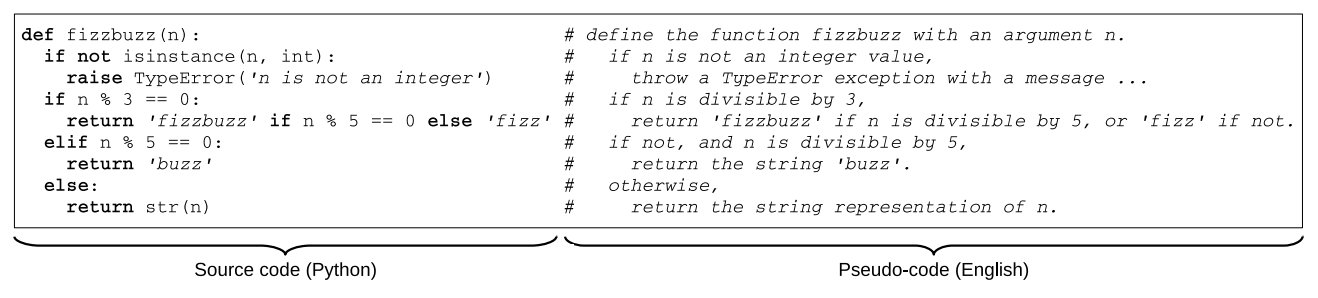
\includegraphics[scale=0.52]{assets/odaetal.png}
    \caption{Example of source code written in Python and corresponding pseudocode created by Pseudogen.}
    \label{pseudogenExample1}
\end{figure}

What the examples in the 2015 paper, as well as a video on their website show,~\footnote{The Pseudogen website can be found at \url{https://ahclab.naist.jp/pseudogen/}} is really a line-for-line translation to English. This could be desired in cases where business people on a team are particularly curious about what the product is really doing under the hood (without having to refactor the code base to Cobol). \\

However, since Pseudogen will translate each line in a servile manner, all error handling is translated too. \Cref{Error handling in Python.} shows some error handling in Python, and \Cref{Error handling in Pseudogen.} shows the result from transpiling it with Pseudogen. The result is considerably more verbose, which defeats some of the point with Python, whose syntax tends to be elegant and succinct, already closely resembling natural language. \\

\begin{lstlisting}[caption={Error handling in Python.}, captionpos=b, label={Error handling in Python.}]
except ValueError as e:
    print(e)
\end{lstlisting}

\begin{lstlisting}[caption={The result of transpiling the code in \Cref{Error handling in Python.} with Pseudogen}, captionpos=b, label={Error handling in Pseudogen.}]
# If ValueError, renamed to e, exception is caught.
    # Call the function print with an argument e.
\end{lstlisting}

Another example is visible in \Cref{listComprehensionPython} and \Cref{listComprehensionPseudogen}, where list comprehension has been translated quite literally. It is plausible to assume people with backgrounds in academia might favour the Python version to the transpiled one, as it closely resembles how we would write set comprehension in mathematics~\cite[kapittel 1 et sted, har ikke boka foran meg:/]{setComprehension}. \\

\begin{lstlisting}[caption={A list comprehension of applying f(n) to integers in the range -10 to 10, and placing the results in a list.}, captionpos=b, label={listComprehensionPython}]
a = [f(n) for n in range(-10, 10)]
\end{lstlisting}

\begin{lstlisting}[caption={The result of transpiling the code in \Cref{listComprehensionPython} with Pseudogen}, captionpos=b, label={listComprehensionPseudogen}]
# Call the function f with an argument n for every
  n in range of integers from range 10 negative
  integer 10, substitute the result for a
\end{lstlisting}

Pseudogen does seem like an excellent tool for translating Python to English, and shows that something like this is indeed possible. However, it is clear that the target audience for its output formats must be people with little to no experience with reading and writing code. Psnodig's intended target audience is somewhat broader, and therefore we believe Pseudogen alone is not enough to solve the problem we are dealing with.

\subsubsection{PseudoEditor}

\forsup{Har ikke fått denne til å funke enda! Synes ikke den gir ikke mening i det hele tatt. Gjerne sjekk den ut på \url{https://pseudoeditor.com/app/}. Selv ikke å poste eksemplet fra \url{https://pseudoeditor.com/guides/merge-sort} fungerer..}

\forsup{Føler derimot at jeg bør ha flere enn ett eksempel på 'source code -> pseudocode'. Eller?}

\subsection{Source Code to Flowcharts}

Even though research argues for the good effects of flowcharts in computer science, there have been few documented efforts towards developing a tool that can effectively translate source code to flowcharts. However, there does exist some software that lets us write flowcharts through a DSL, and we will look at two of them.

\subsubsection{Naive Approach}

Yet again, calling it a naive approach might not be entirely accurate, but manually translating our code to flowcharts does introduce some intricacies. For one, like with TBP, we have to maintain both versions, and if we change too much of our main idea, then the time spent on making the IBP version is - to a certain extent - wasted. \\

Another flaw is that we have to spend time thinking about how the flowchart should look like, which parts could and should be abstracted, how they should be presented instead (or if they should be removed altogether) etc. Which colours should the frames have? How should the arrows look? Which font should be used? By automating this process, we do not have to worry about details unrelated to the actual program logic. \\

The perk of doing it this way, however, is that we can do it entirely our way. We can choose which tools we want to use, and if we are already proficient in making flowcharts based on source code, then this actually seems like a natural choice. If we also like spending time on details like colours, fonts, shapes etc., then at least the naive approach does not limit our creativity in any way. \\

\forsup{Jeg føler egentlig at det er best å starte med det positive, og avslutte med det negativel. Hva tenker dere?}

\subsubsection{Code2Flow}

Code2Flow is a tool that lets us create flowcharts with natural language, decorated with a C-inspired syntax. Their website states that we might get away with pasting syntactically correct C programs, but that this is purely incidental. This goes to show that the Code2Flow team have indeed developed a DSL with their own syntax. \\

Flowcharts created with Code2Flow have a few, consistent colours to differentiate parts of their corresponding programs. Start- and end expressions are displayed as red ovals, while all remaining expressions are displayed as blue rectangles. Conditionals, loops and match statements are displayed with red rhombuses, and comments are displayed with orange rectangles. \\

\begin{lstlisting}[caption={A Code2Flow program.}, captionpos=b, label={A Code2Flow program.}]
First expression;
Another expression;
if (conditional) {
  expression 1;
} else {
  expression 2; // Random comment
}
Last expression;
\end{lstlisting}

\Cref{A Code2Flow program.} shows a program written with Code2Flow, and \Cref{A Code2Flow flowchart.} presents the corresponding flowchart. As we can see, syntactically correct expressions are any combination of UTF-8 characters. Code2Flow will never warn us about syntactic errors, and will \textit{always} try to construct whatever flowchart it can. In turn, there is no clear way to test a Code2Flow program. \\

\begin{figure}[ht]
    \centering
    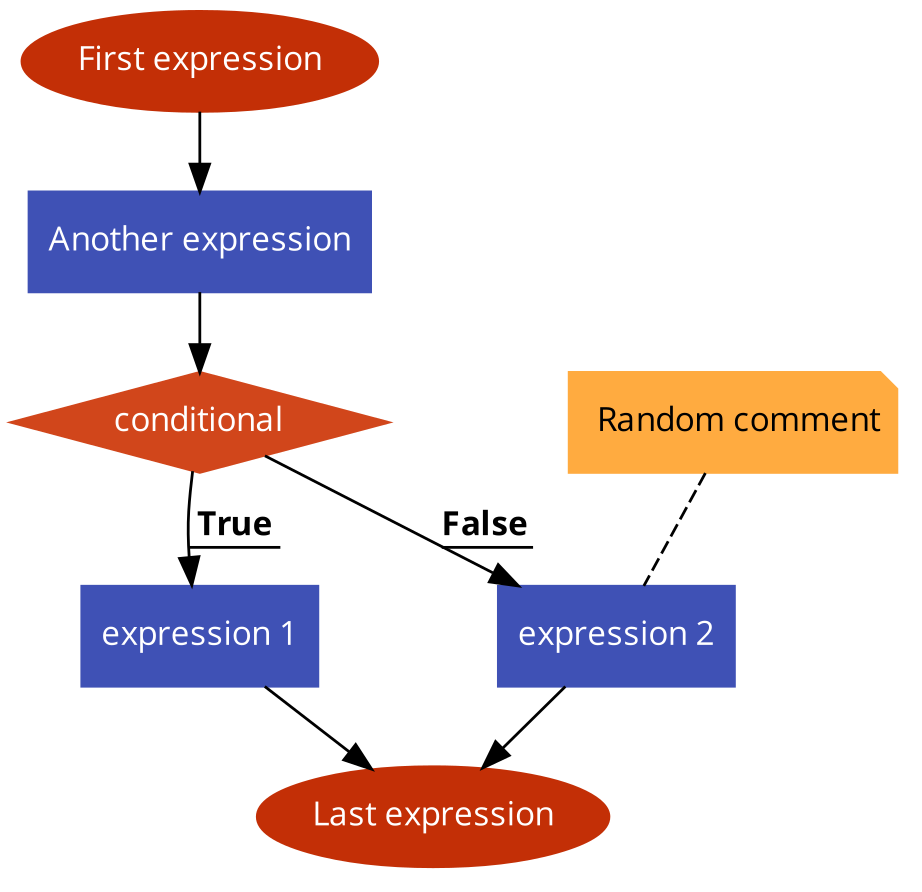
\includegraphics[scale=0.2]{assets/code2flow_example.png}
    \caption{The resulting flowchart from transpiling the Code2Flow code in \Cref{A Code2Flow program.}}
    \label{A Code2Flow flowchart.}
\end{figure}

If our C program inadvertently creates a ``correct'' flowchart, we can use a C compiler to test said program on the side. However, future changes to the C program are not guaranteed to successfully transpile to a new flowchart.

\subsubsection{Mermaid.js}

Mermaid.js is a DSL for rendering diagrams (including flowcharts) from a Markdown-inspired syntax. Even though we can construct many different diagrams with Mermaid.js, we will focus on the flowcharts. Like Code2Flow, they render flowcharts in real time. However, Mermaid.js \textit{will} warn us about syntax errors, and only re-render syntactically correct programs. \\

To construct a Mermaid.js flowchart, our source program must start with \texttt{flowchart TD}. Nodes can come in many different shapes, and are denoted by the types of brackets they use. For instance, \texttt{Node[ ]} displays a rectangle, \texttt{Node(( ))} displays a circle, and \texttt{Node\{ \}} displays a rhombus. Edges also come in many shapes: \texttt{$--$>} displays an arrow, \texttt{-.->} displays a dotted arrow, whilst \texttt{$---$} will display a simple link. \\

We can also add text to our nodes, by placing it within the brackets, like \texttt{Node[text]}. Arrows can also include text by breaking them up into two parts, like \texttt{$--$ text $--$>}.~\footnote{The full documentation can be found at~\url{https://mermaid.js.org/syntax/flowchart.html}} \\

\begin{lstlisting}[caption={A mermaid.js program.}, captionpos=b, label={A mermaid.js program.}]
flowchart TD
    A([First expression])
        --> B[Another expression]
    B --> C{contidional}
    C -- True --> D[Expression 1]
    C -- False --> E[Expression 2]
        %% Random comment
    D --> F([Last expression])
    E --> F
\end{lstlisting}

Just like with Code2Flow, the text inside these nodes can be anything. \Cref{A mermaid.js program.} shows a program written with Mermaid.js, and \Cref{A mermaid.js flowchart.} shows the corresponding flowchart. Contrary to Code2Flow, comments are ignored by the parser, and solely exist to aid the programmer. They must also be on their own lines. \\

\begin{figure}[ht]
    \centering
    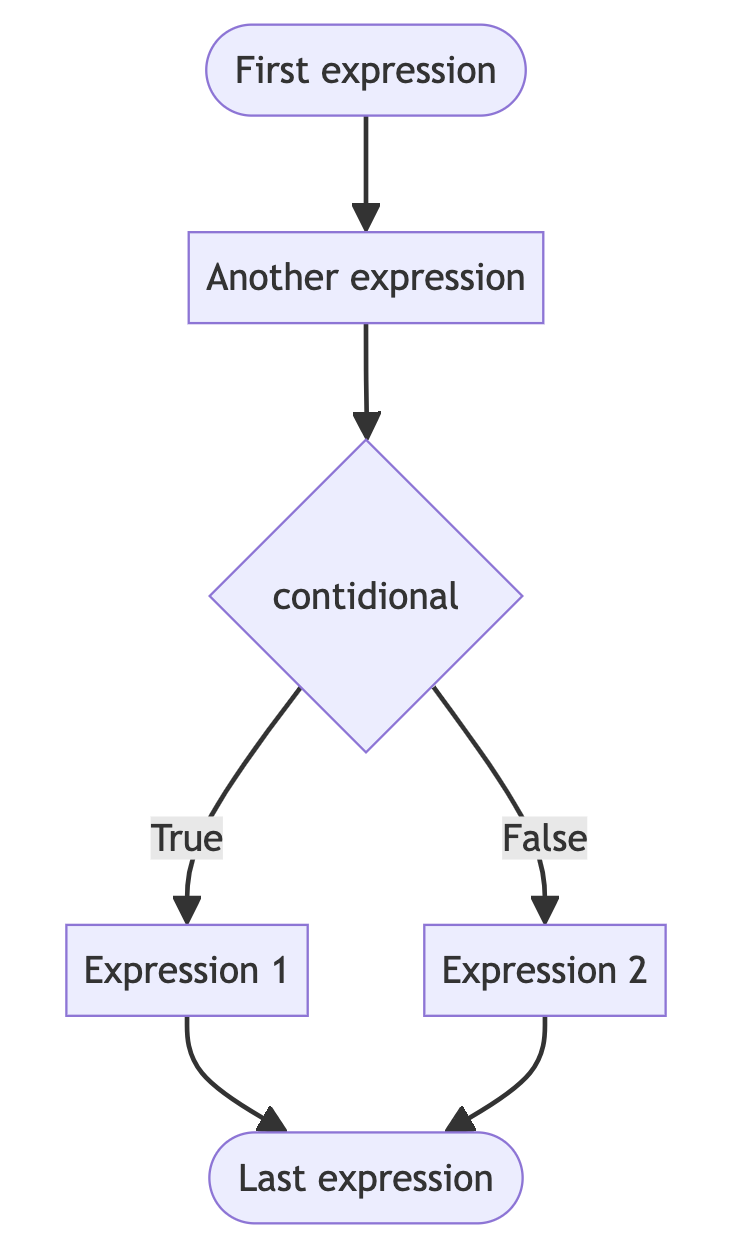
\includegraphics[scale=.4]{assets/mermaidjs.png}
    \caption{The resulting flowchart from transpiling the Mermaid.js code in \Cref{A mermaid.js program.}}
    \label{A mermaid.js flowchart.}
\end{figure}

The biggest drawback of Mermaid.js is that the syntax is very different from any programming language. This means pasting our source code will not yield any result, and we have to carefully translate our code every time. This means that it is fully our responsability to maintain the abstraction level we want. Like Code2Flow, Mermaid.js has no way of letting us test the code either.
